\documentclass[11pt,a4paper]{article}
\usepackage[margin=27mm]{geometry}
\usepackage{pdfpages,hyperref}
\pdfinclusioncopyfonts=1
\title{Primitive geometries from subgroup pairs\\Proofs and source comparison}
\author{Human Compression project}\date{}
\begin{document}\maketitle
This volume treats the fixed twelve-page 2019 article
\emph{On primitive geometries of rank two}, by Dimitri Leemans and
Bernardo G. Rodrigues. Its original Rudvalis total is false. The complete
mathematical treatment consists of the opening synthesis and the six
proofs listed below, together with their finite certificates and explicit
classification premises.

\begin{enumerate}
\item Complete source treatment and the common parameter set (4 pages).
\item The accepted Rudvalis principal correction (2 pages).
\item Counting subgroup pairs from fixed points (3 pages).
\item The five character calculations (2 pages).
\item The six outer-automorphism counts and five suborbit tables (4 pages).
\item The general coset-action algorithm correction (2 pages).
\item All 37 M11 geometries and 70 design entries (6 pages).
\end{enumerate}

The earlier component texts retain their accepted local scopes. Their
statements about obligations outside their individual components are
resolved by the other proofs in this volume, as the opening synthesis
explains. The M11 publication edition corrects our section citation and
uses a plain heading; its mathematical content is unchanged. Exact
originals and the textual deltas remain available in the accompanying
certificate.

The original paper, prior classifications and library data are attributed
inputs. The electronic representative files linked by the authors have
not been verified. This volume supplies a complete mathematical parameter
set and verifies all finite tables printed in the fixed article; it does
not publish an expanded catalogue of all 568220 representatives. No Lean
formalization, new principal-refutation credit or compression measurement
is claimed.
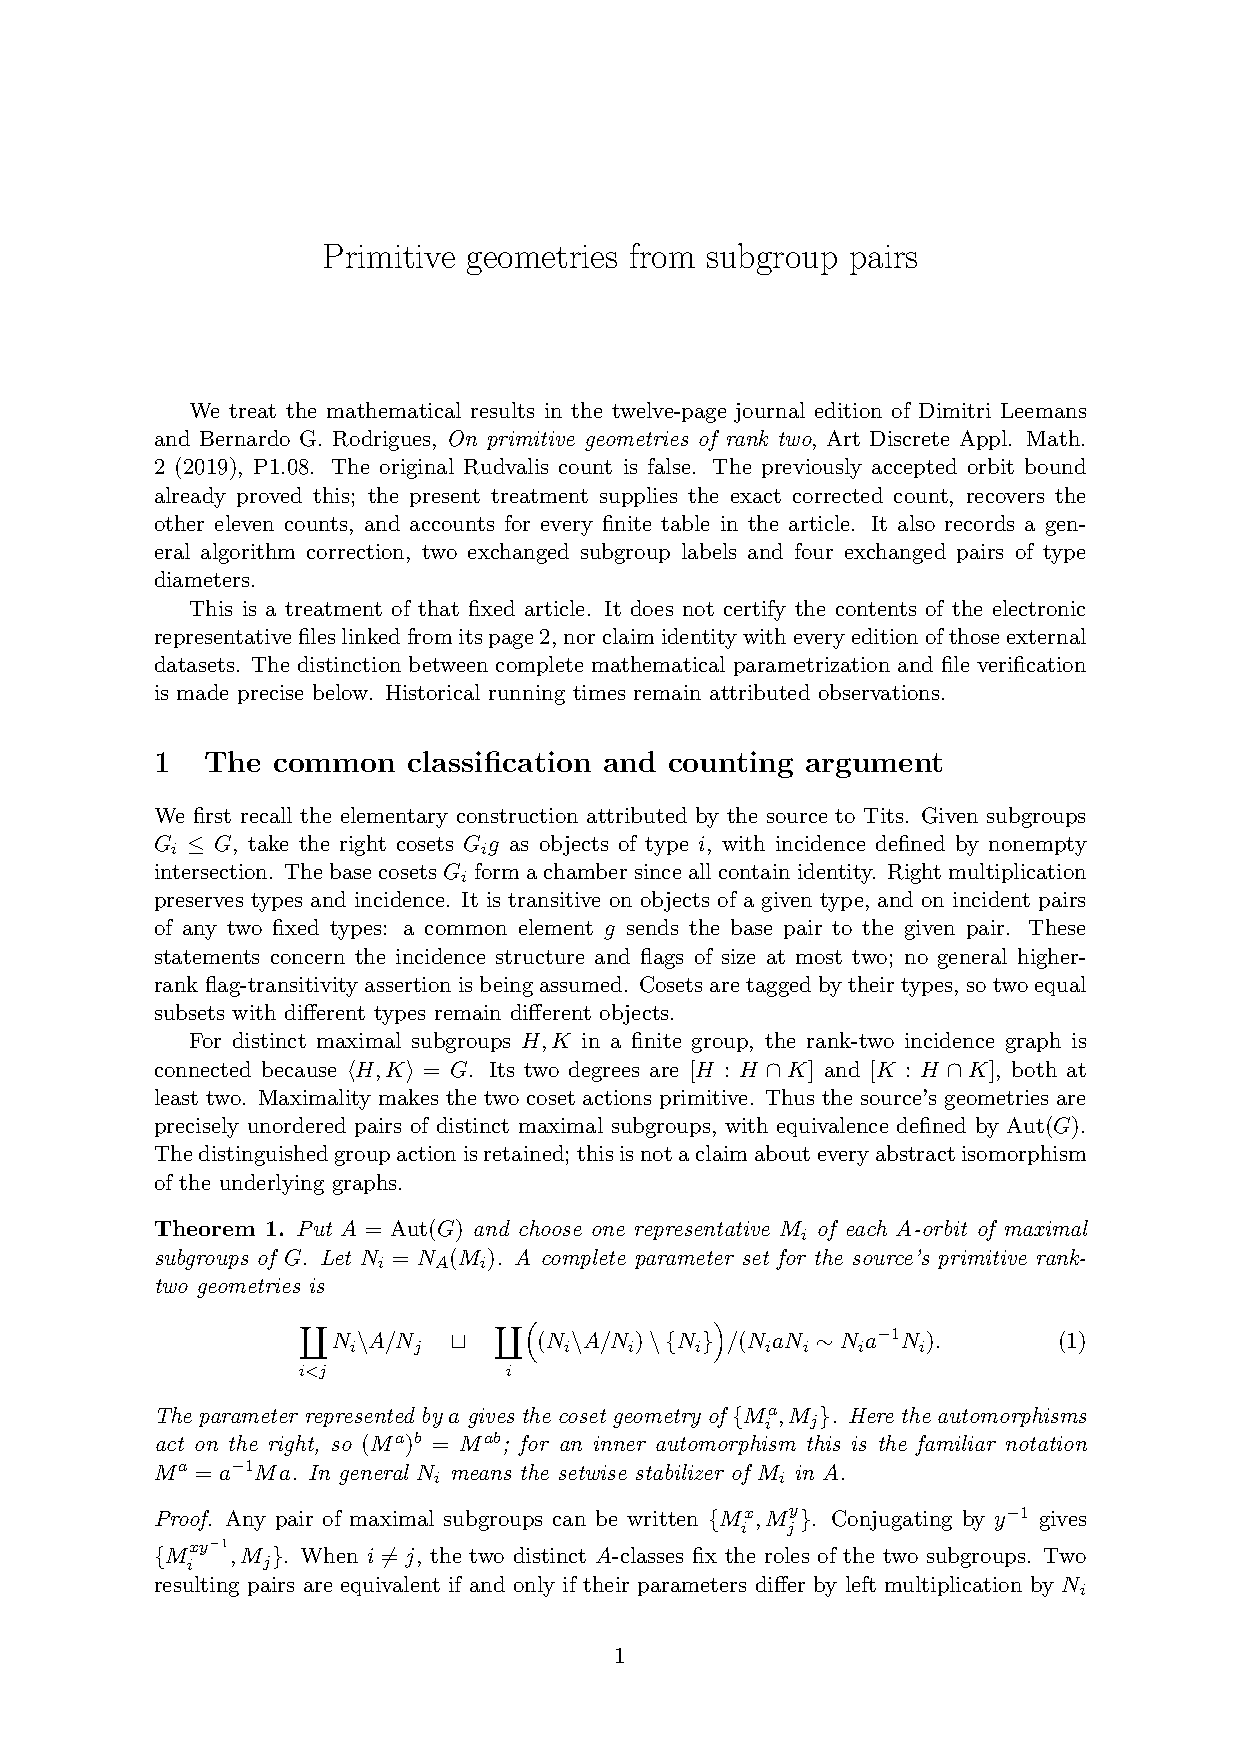
\includepdf[pages=-]{completion.pdf}
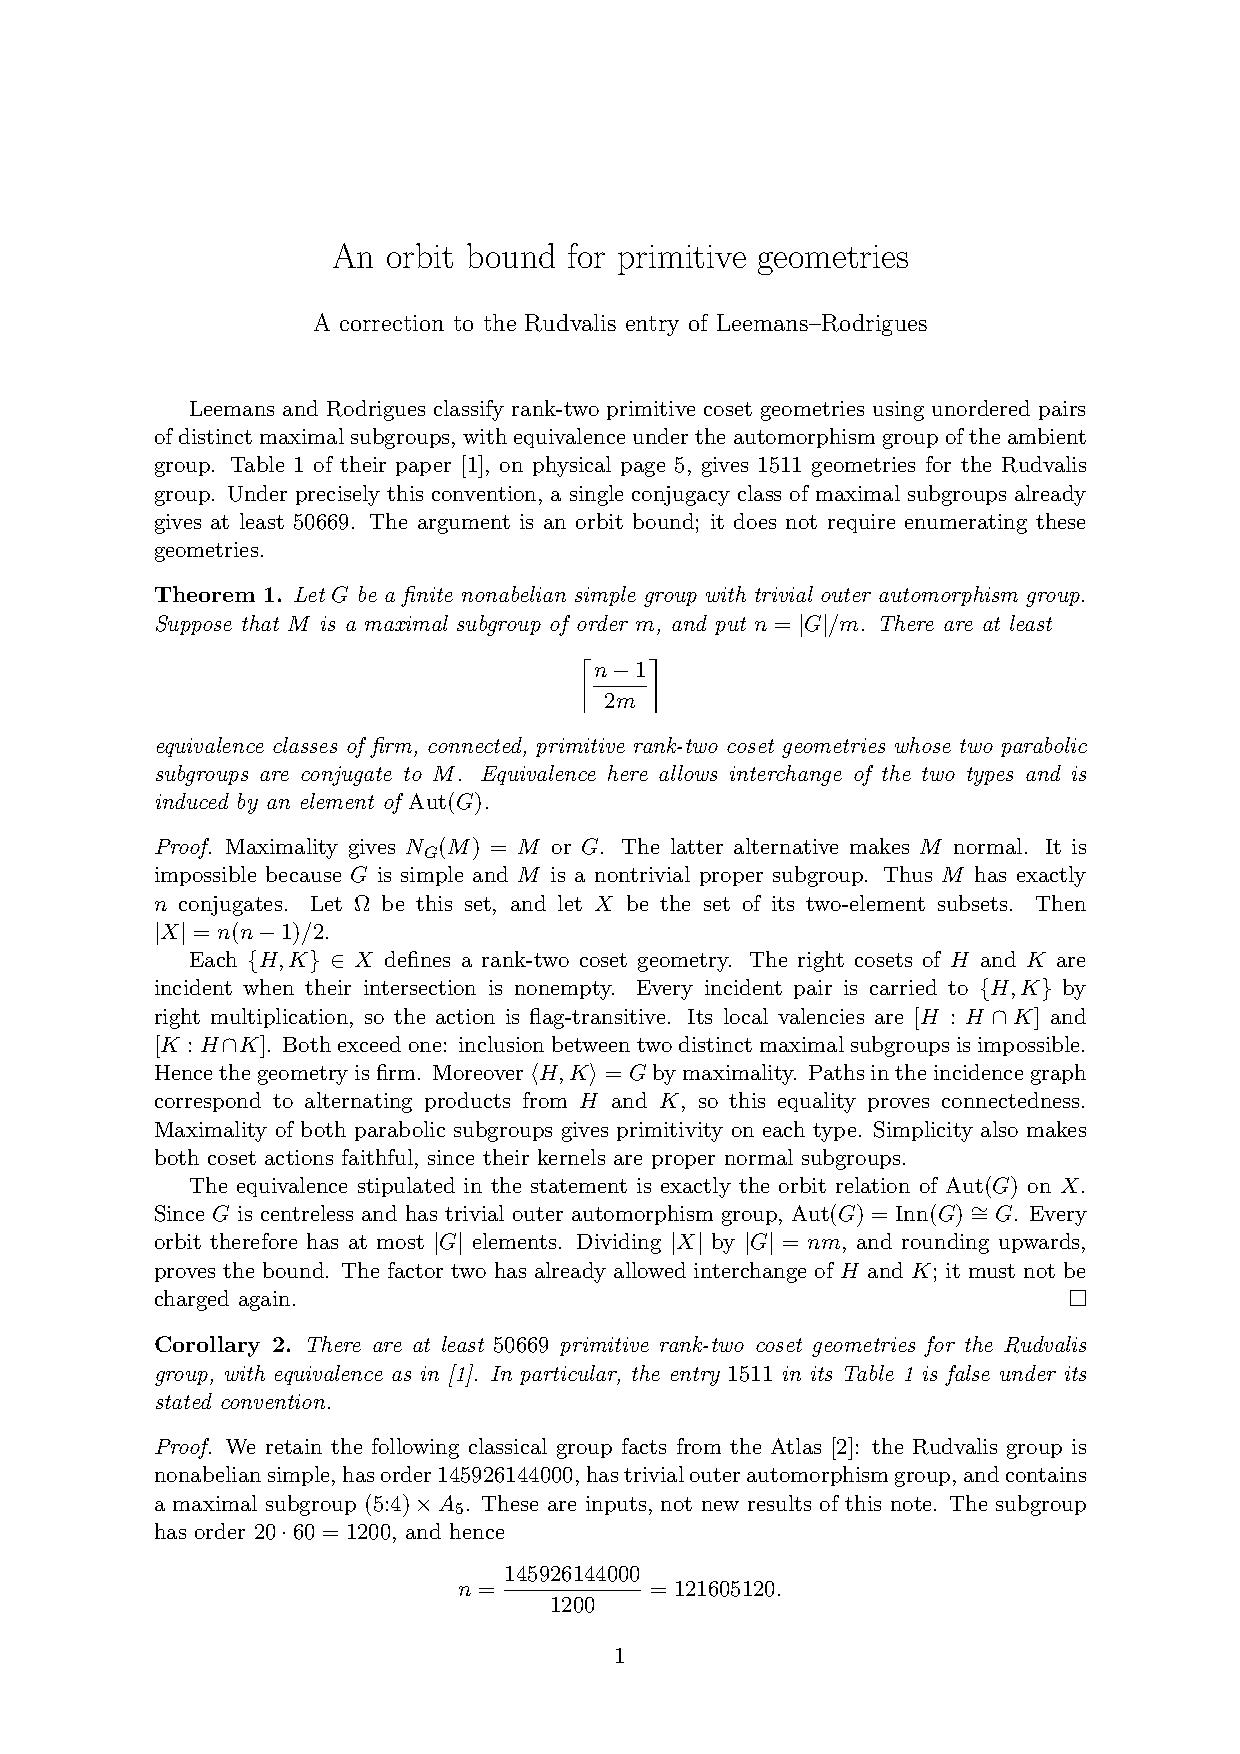
\includepdf[pages=-]{proofs/principal.pdf}
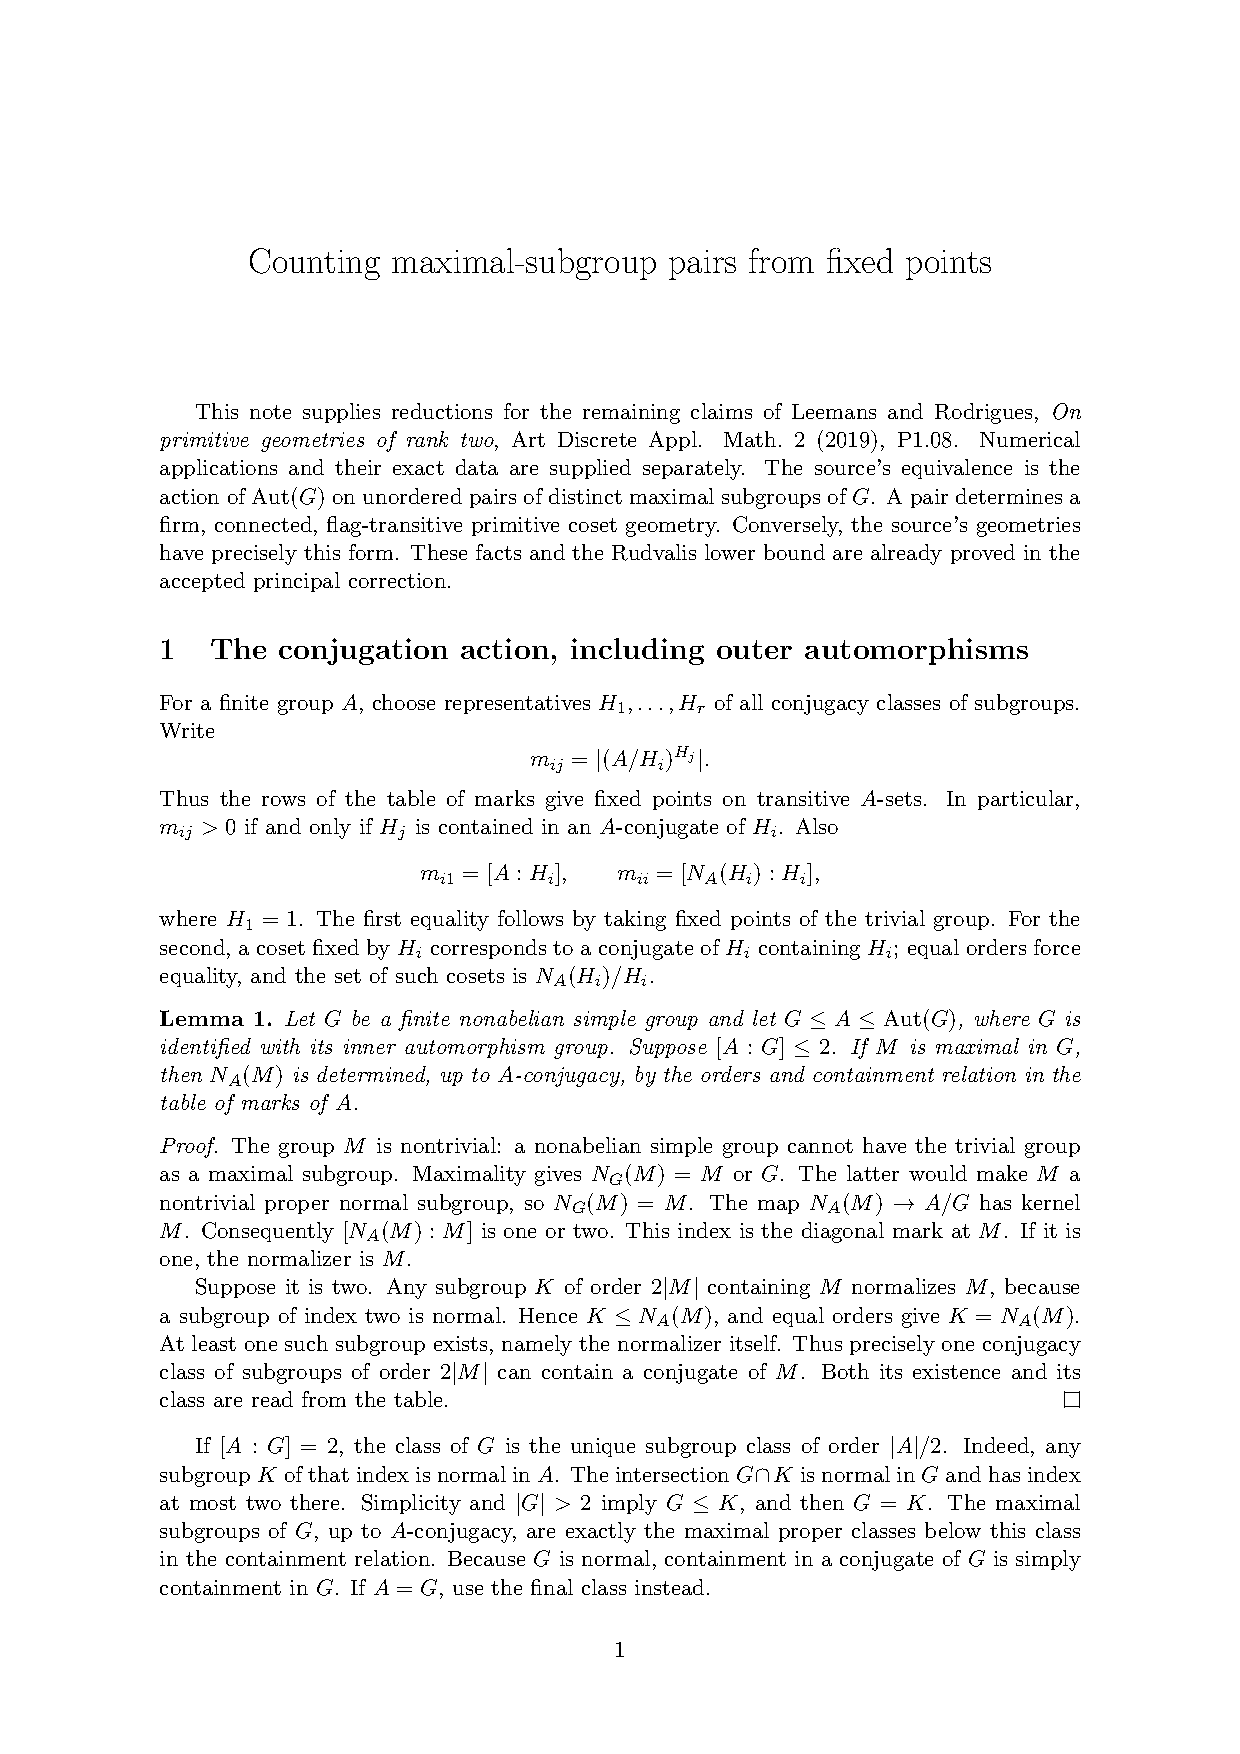
\includepdf[pages=-]{proofs/theory.pdf}
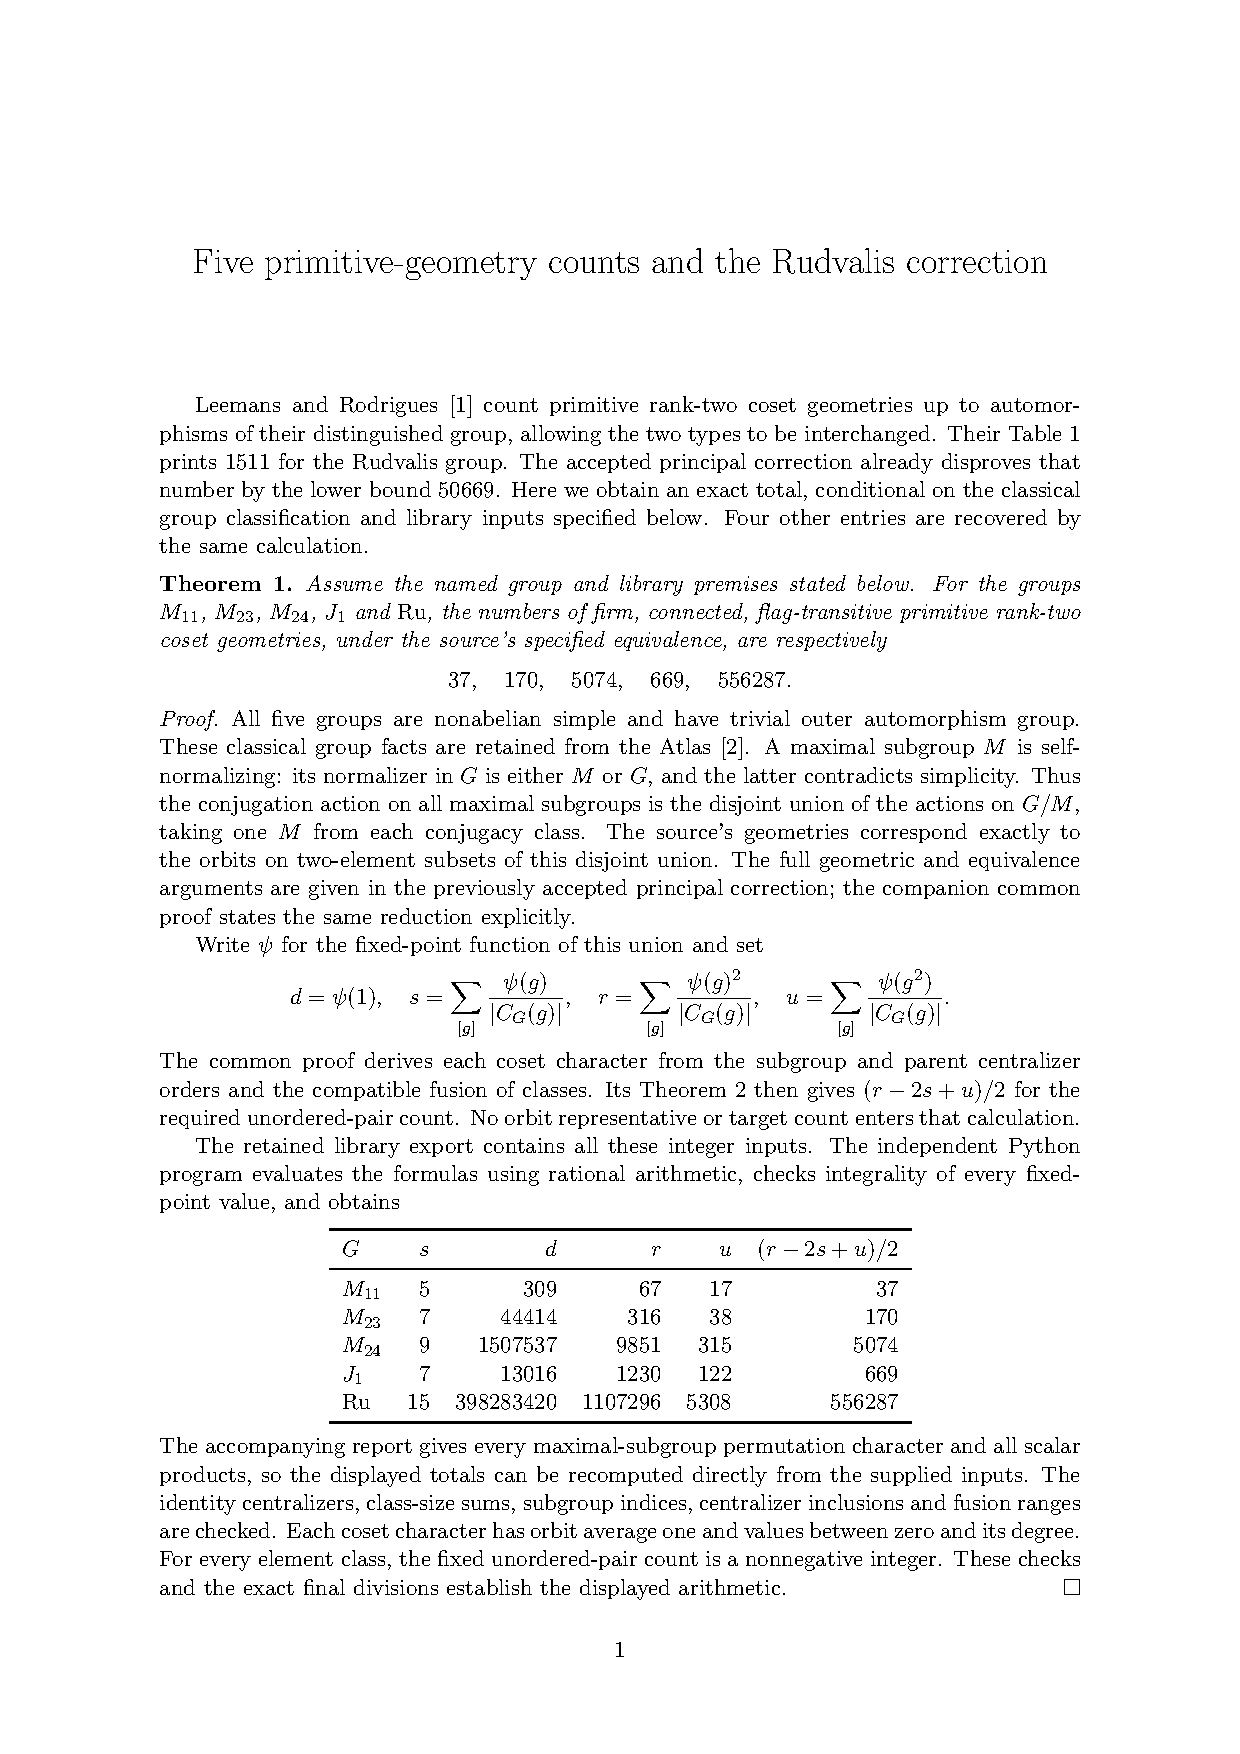
\includepdf[pages=-]{proofs/characters.pdf}
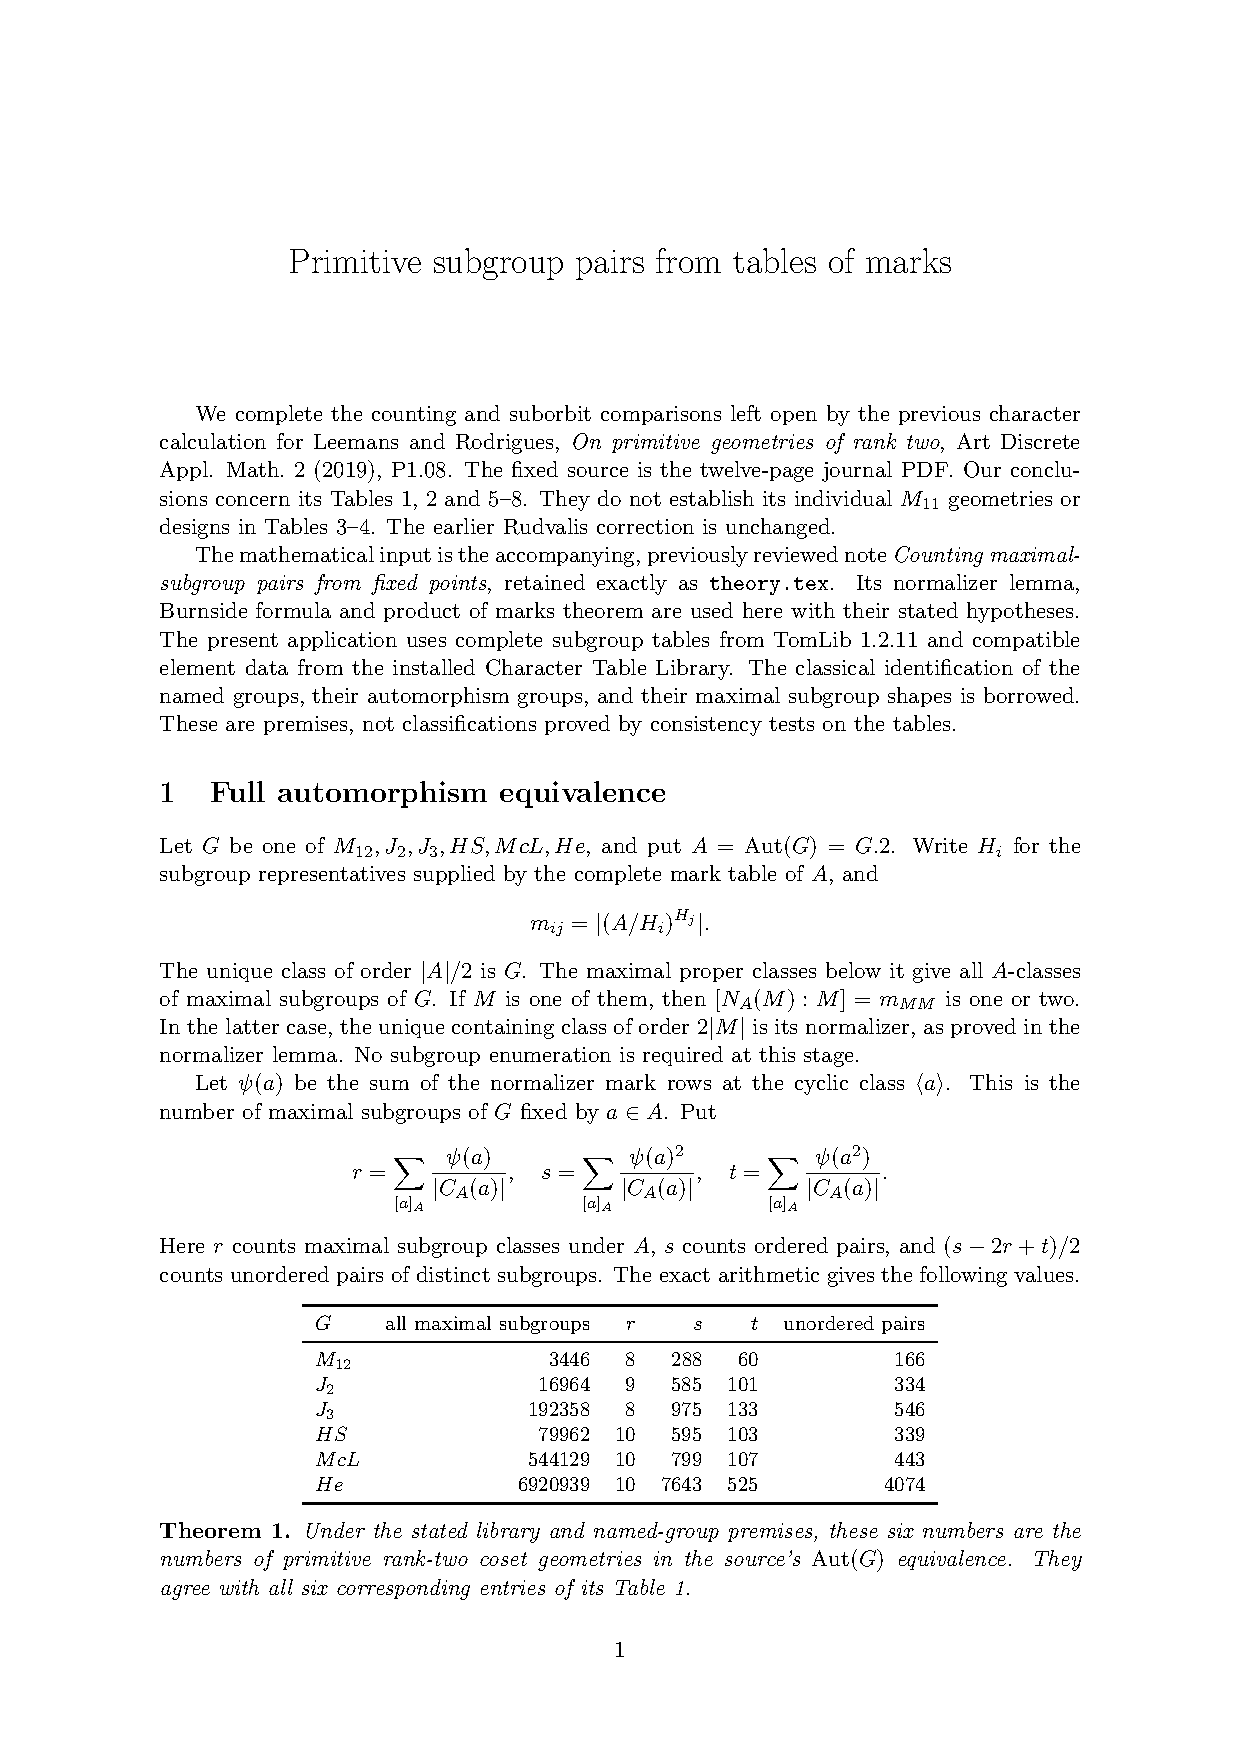
\includepdf[pages=-]{proofs/marks.pdf}
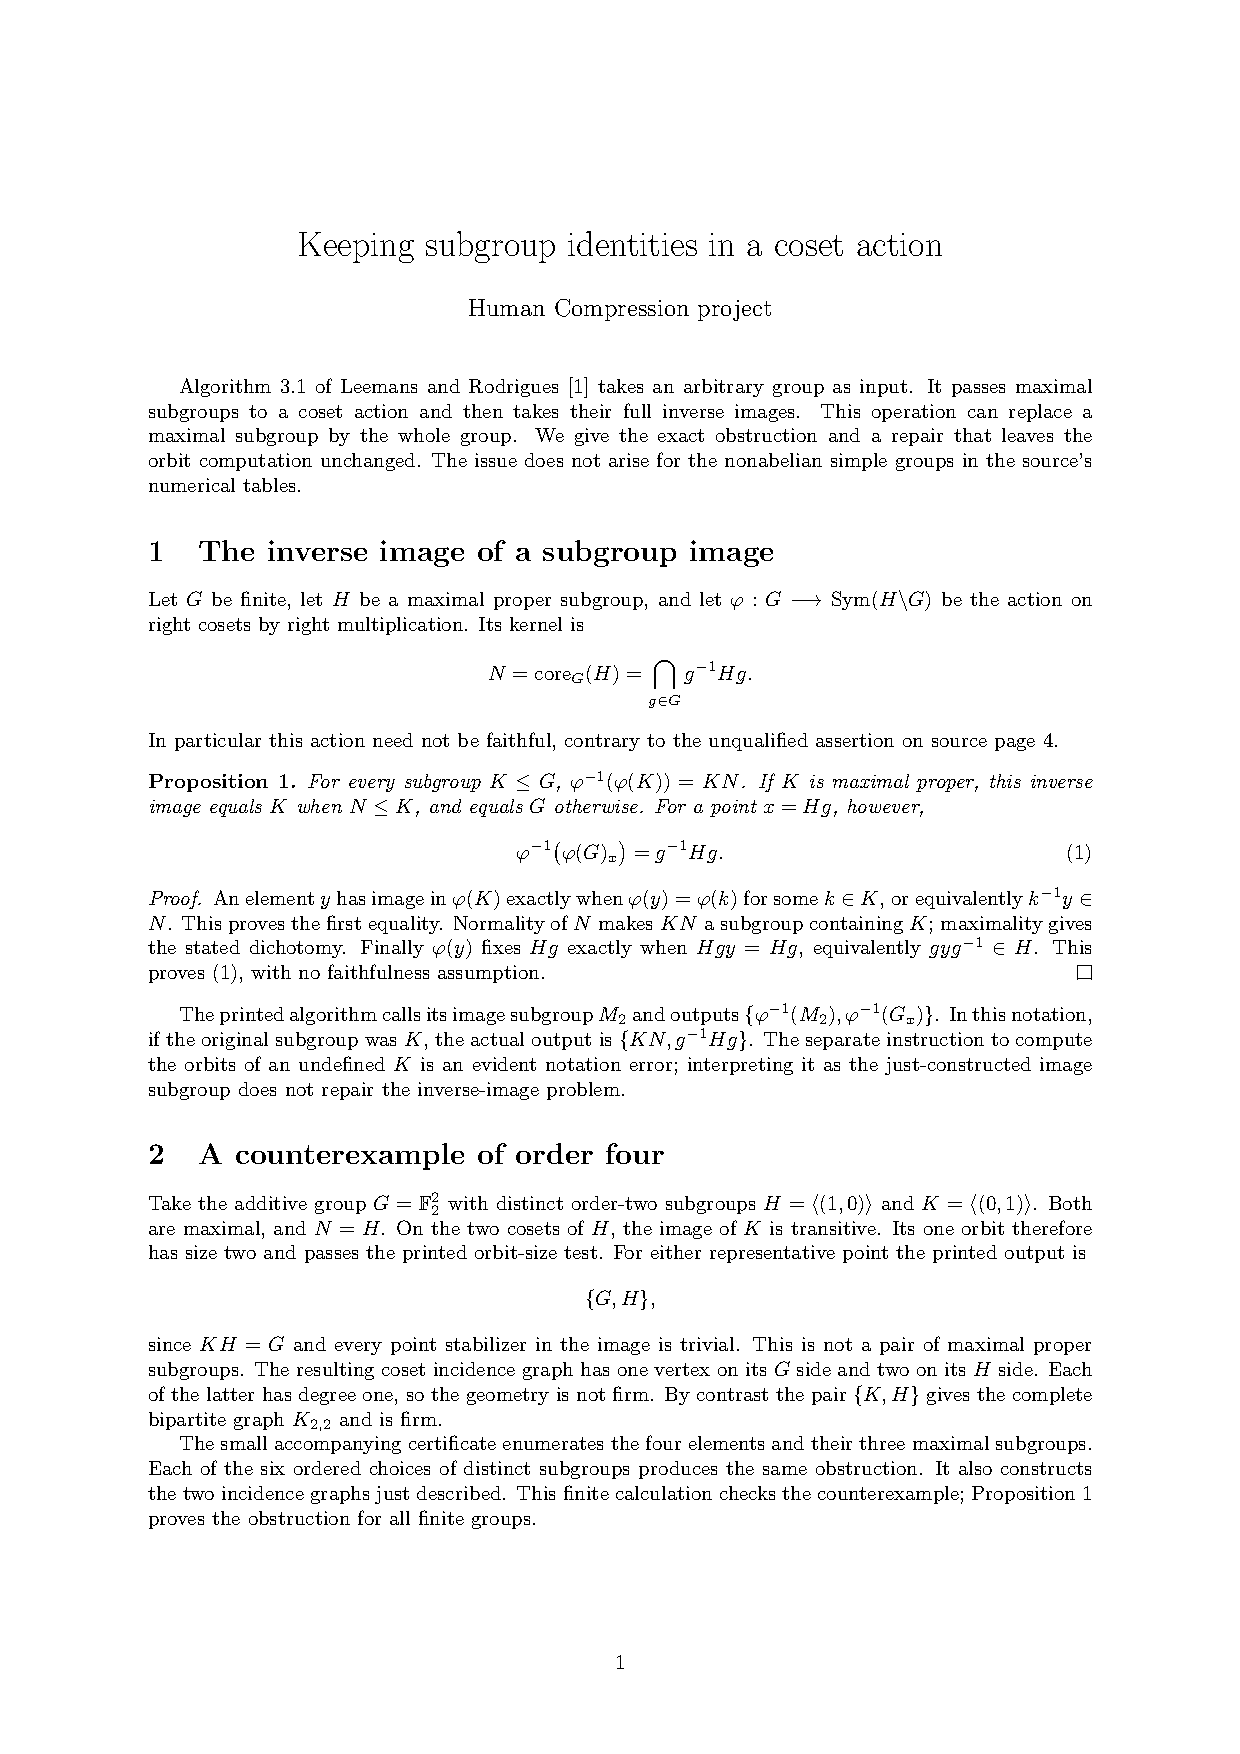
\includepdf[pages=-]{proofs/algorithm.pdf}
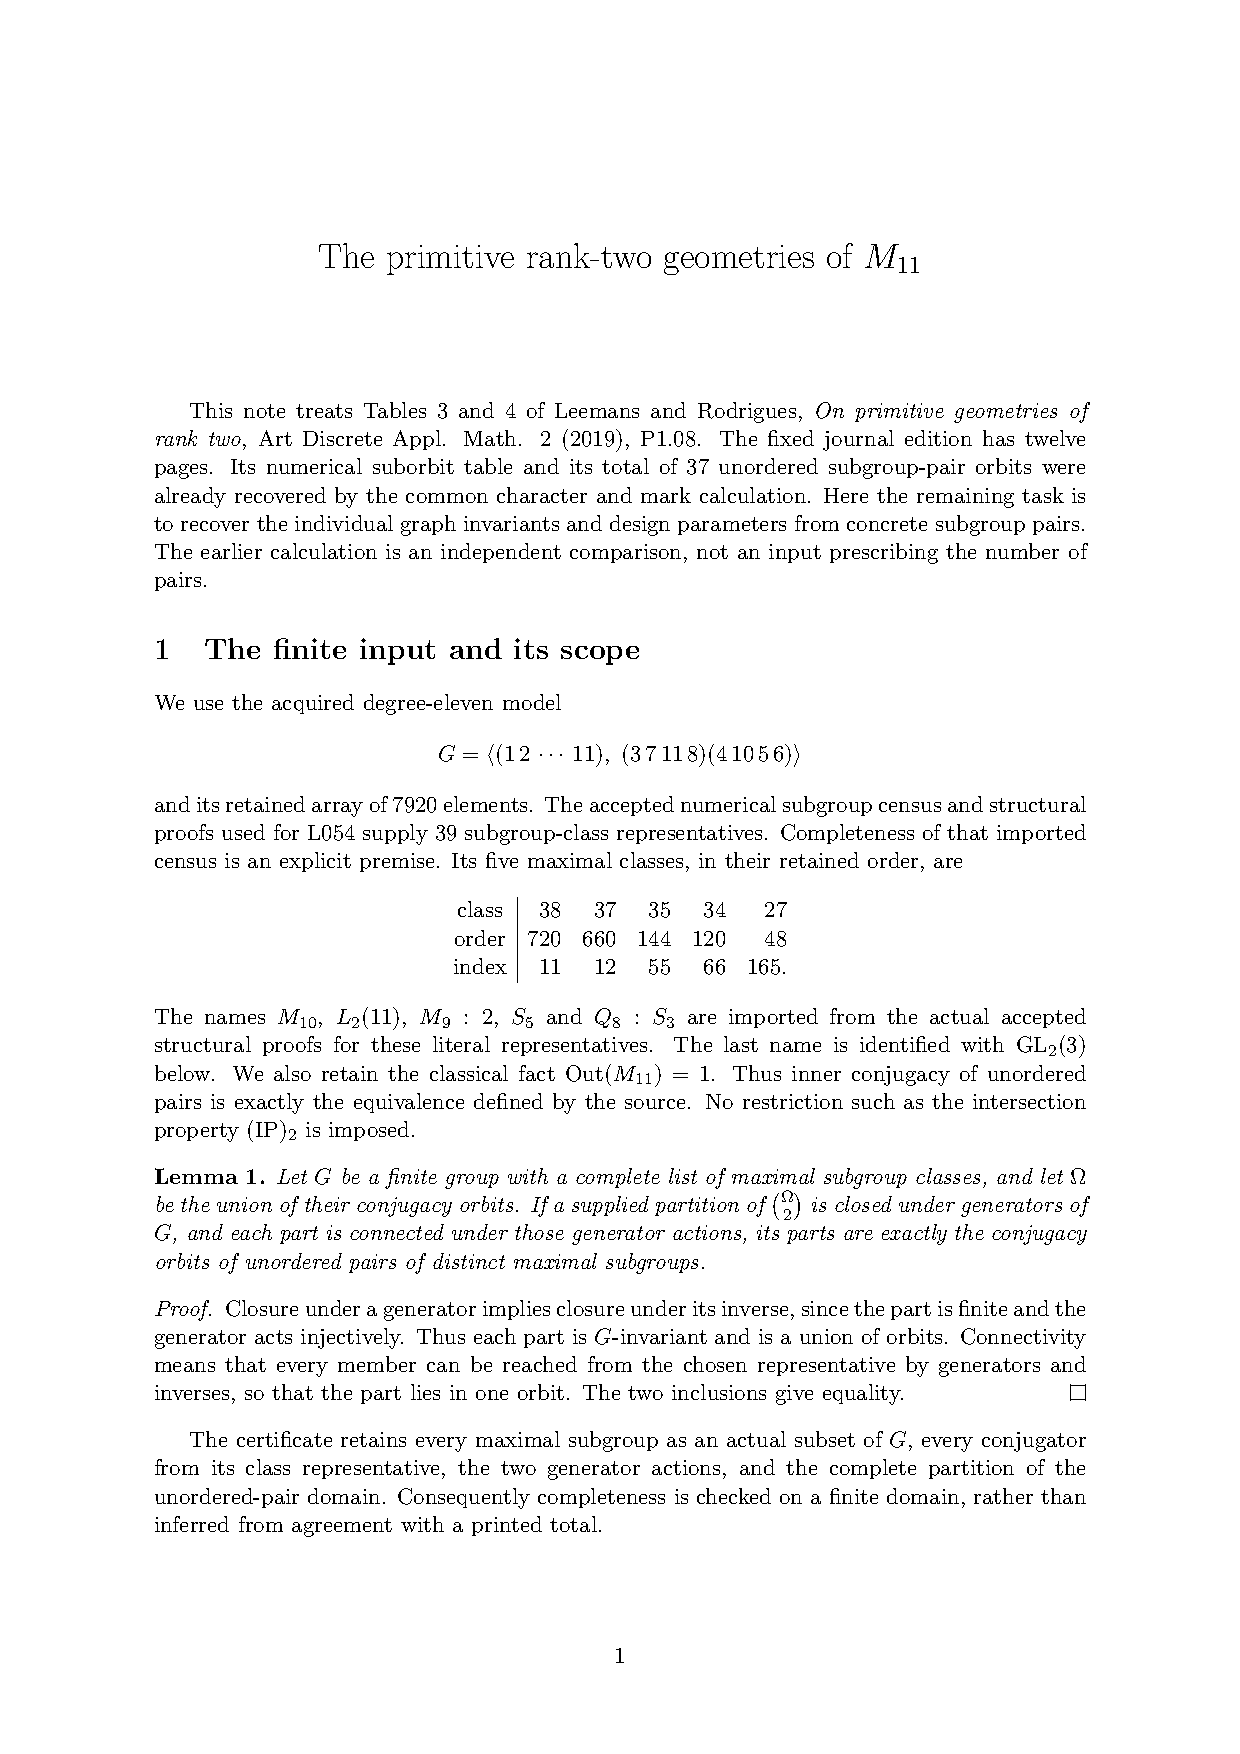
\includepdf[pages=-]{proofs/m11.pdf}
\end{document}
